\chapter{边界共形场论}
本章讨论带边Riemann面(例如带,圆环)上的共形场论,也就是边界共形场论,之后用缩写BCFT指代。这个理论能用来研究带边物理系统的临界现象,在D膜和超弦理论中也有重要应用。本章,我们先讨论以实轴为边界的上半平面上的CFT中的关联函数,接着讨论圆环上的CFT的配分函数及其在模变换下的行为。
\section{ 两点函数}
在复平面 $\mathbb{C} $上的CFT中,初级场两点和三点函数的形式可从全局共形对称性确定。我们已经看到,全局共形对称性不能完全确定住四点函数的形式,由此不能知道它具体如何依赖于交比。在带边Riemann面上是什么样呢?Cardy\footnote{J. L. Cardy, Nucl. Phys. B 240 (1984) 514.}\footnote{J. L. Cardy, Nucl. Phys. B 275 (1986) 200.}思考过这些问题,并写过综述\footnote{J. L. Cardy, arXiv:hep-th/0411189.}\footnote{J. L. Cardy, arXiv:math-ph/0103018.}。

考虑上半复平面
\begin{equation}
	H=\{z=x+i y \in \mathbb{C} ; y>0\}
\end{equation}
上的共形场论。$ H$ 的边界是实轴$ \mathbb{R}$ , $H$ 内的点有时称为体(bulk)中的点。
\begin{figure}[h]
	\centering
	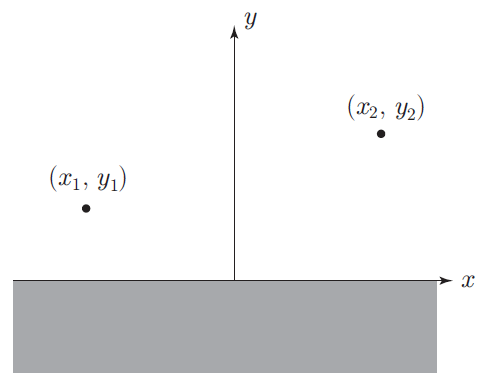
\includegraphics[width=0.6\linewidth]{fig/7.1.png}
	\caption{上半复平面上的CFT中的两点函数。}
\end{figure}
在 $H $内的点上,初级场的定义和复平面上一样。简单起见,考虑共形权为 $(h, h)$ ,自旋为零的初级场$ \phi(z, \bar{z})$ 的两点函数
$$
\left\langle\phi\left(z_{1}, \bar{z}_{1}\right) \phi\left(z_{2}, \bar{z}_{2}\right)\right\rangle
$$
如图7.1。

在Riemann球面上,也就是复平面 $\mathbb{C} $加上无穷远点,全局共形变换是 $PSL(2, \mathbb{C}) $变换
$$
z \rightarrow z^{\prime}=\frac{a z+b}{c z+d}, \quad a d-b c=1, \quad a, b, c, d \in \mathbb{C}
$$
$H $上的全局共形变换必须保持边界的形状,将实轴上的点映到实轴上,因此 $a,b,c,d $必须是实数。这些变换是$ PSL(2, \mathbb{R}) $变换
\begin{equation}
z \rightarrow z^{\prime}=\frac{\alpha z+\beta}{\gamma z+\delta}, \quad \alpha \delta-\beta \gamma=1, \quad \alpha, \beta, \gamma, \delta \in \mathbb{R}
\end{equation}
无穷小变换分为实轴上的平移,标度变换和特殊共形变换
\begin{align} &z \rightarrow z^{\prime}=z+\epsilon_{-1}\\ &z \rightarrow z^{\prime}=z+\epsilon_{0} z\\ &z \rightarrow z^{\prime}=z+\epsilon_{1} z^{2} \end{align}
这里 $\epsilon_{-1}, \epsilon_{0}, \epsilon_{1} $是实数。$ H $上的共形变换受更多限制,因而对称性对关联函数的限制更少。

全局共形变换下,对两点函数有Ward恒等式
\begin{equation}
	\begin{aligned} \left\langle\phi\left(z_{1}, \bar{z}_{1}\right) \phi\left(z_{2}, \bar{z}_{2}\right)\right\rangle=&\left.\left.\prod_{i=1,2}\left(\frac{d z^{\prime}}{d z}\right)^{h}\right|_{z=z_{i}}\left(\frac{d \bar{z}^{\prime}}{d \bar{z}}\right)^{h}\right|_{\bar{z}=\bar{z}_{i}} \\ & \times\left\langle\phi\left(z_{1}^{\prime}, \bar{z}_{1}^{\prime}\right) \phi\left(z_{2}^{\prime}, \bar{z}_{2}^{\prime}\right)\right\rangle \end{aligned} 
\end{equation}
令$ z_{i}=x_{i}+i y_{i} $( $i=1,2$ ),那么两点函数是$ \left(x_{1}, y_{1}, x_{2}, y_{2}\right)$ 的函数。 $x $方向上的平移对称性要求它是 $x_1-x_2 $的函数:
$$
\left\langle\phi\left(z_{1}, \bar{z}_{1}\right) \phi\left(z_{2}, \bar{z}_{2}\right)\right\rangle=G\left(x_{1}-x_{2}, y_{1}, y_{2}\right)
$$
注意,由于存在边界,$ y$ 方向上没有平移对称性。接着,在标度变换
\begin{equation}
	\begin{aligned} &x \rightarrow x^{\prime}=(1+\epsilon) x \\ &y \rightarrow y^{\prime}=(1+\epsilon) y \end{aligned} 
\end{equation}
下,两点函数满足
\begin{equation}
	G\left(x_{1}-x_{2}, y_{1}, y_{2}\right)=(1+\epsilon)^{4 h} G\left(x_{1}^{\prime}-x_{2}^{\prime}, y_{1}^{\prime}, y_{2}^{\prime}\right) 
\end{equation}
记 $u=x_{1}-x_{2}$ ,在$ \epsilon$ 很小时展开得到
\begin{equation}	
4 h G+u \frac{\partial G}{\partial u}+y_{1} \frac{\partial G}{\partial y_{1}}+y_{2} \frac{\partial G}{\partial y_{2}}=0 
\end{equation}
于是 $G$ 可写成
\begin{equation}
	G\left(u, y_{1}, y_{2}\right)=\left(y_{1} y_{2}\right)^{-2 h} \psi\left(\xi_{1}, \xi_{2}\right), \quad \xi_{i}=\frac{y_{i}}{u}
\end{equation} 
最后考虑特殊共形变换 $z^{\prime}=z+\epsilon z^{2} $。$ x,y $坐标变换为:
\begin{equation}
	\begin{aligned} &x \rightarrow x^{\prime}=x+\epsilon\left(x^{2}-y^{2}\right)\\ &y \rightarrow y^{\prime}=y+2 \epsilon x y \end{aligned} 
\end{equation}
Jacobian(之积)是
$$
\frac{d z^{\prime}}{d z} \frac{d \bar{z}^{\prime}}{d \bar{z}}=(1+2 \epsilon z)(1+2 \epsilon \bar{z})=1+4 \epsilon x
$$
因而Ward恒等式给出
\begin{equation}
	G\left(u, y_{1}, y_{2}\right)=\left(1+4 \epsilon x_{1}\right)^{h}\left(1+4 \epsilon x_{2}\right)^{h} G\left(u^{\prime}, y_{1}^{\prime}, y_{2}^{\prime}\right)
\end{equation}
展开得到
\begin{equation}
	\begin{aligned} &\left(x_{1}^{2}-x_{2}^{2}-y_{1}^{2}+y_{2}^{2}\right) \frac{\partial G}{\partial u}+2 x_{1} y_{1} \frac{\partial G}{\partial y_{1}}+2 x_{2} y_{2} \frac{\partial G}{\partial y_{2}} \\ &+4\left(x_{1}+x_{2}\right) h G=0 \end{aligned} 
\end{equation}
与标度变换的方程 (7.9) 联立,得到
\begin{equation}
	\left(y_{2}^{2}-y_{1}^{2}\right) \frac{\partial G}{\partial u}+u\left(y_{1} \frac{\partial G}{\partial y_{1}}-y_{2} \frac{\partial G}{\partial y_{2}}\right)=0 
\end{equation}
代入 (7.10) 给出
\begin{equation}
	\left(\xi_{1}^{2}-\xi_{2}^{2}+1\right) \xi_{1} \frac{\partial \psi}{\partial \xi_{1}}+\left(\xi_{1}^{2}-\xi_{2}^{2}-1\right) \xi_{2} \frac{\partial \psi}{\partial \xi_{2}}=0 
\end{equation}
解得
\begin{equation}
	\psi\left(\xi_{1}, \xi_{2}\right)=\Psi\left(\frac{\left(\xi_{1}+\xi_{2}\right)^{2}+1}{\xi_{1} \xi_{2}}\right) 
\end{equation}
总结一下,$ H$ 上的两点函数形如
\begin{equation}
	\left\langle\phi\left(z_{1}, \bar{z}_{1}\right) \phi\left(z_{2}, \bar{z}_{2}\right)\right\rangle=\left(y_{1} y_{2}\right)^{-2 h} \Psi\left(\frac{\left(x_{1}-x_{2}\right)^{2}+\left(y_{1}+y_{2}\right)^{2}}{y_{1} y_{2}}\right)
\end{equation}
全局共形对称性没有完全确定住它的形式,这同复平面上四点函数的情形一样。事实上,复平面上的点 $\left(z_{1}, z_{2}, \bar{z}_{1}, \bar{z}_{2}\right) $间的交比
\begin{equation}
	\eta=\frac{\left(z_{1}-\bar{z}_{1}\right)\left(z_{2}-\bar{z}_{2}\right)}{\left(z_{1}-\bar{z}_{2}\right)\left(z_{2}-\bar{z}_{1}\right)} 
\end{equation}
是实数,并且是 $PSL(2, \mathbb{R}) $不变量。$ \eta$ 用$ x,y$ 坐标写是
\begin{equation}
	\eta=\frac{4 y_{1} y_{2}}{\left(x_{1}-x_{2}\right)^{2}+\left(y_{1}+y_{2}\right)^{2}} 
\end{equation}
正是 (7.17) 右边括号内参数倒数的4倍。一般地, $H$ 上的$ n$ 点函数可同复平面上的$ 2n$ 点函数对应起来。要看到这一关系,基于无穷小共形Ward恒等式来讨论比较方便。
\section{加倍技巧}
考虑 $H$ 上共形权为$ \left(h_{i}, h_{i}\right)$ ,自旋为零的初级场 $\phi_{i}\left(z_{i}, \bar{z}_{i}\right) $( $i=1, \cdots, n$ )的关联函数
$$
\left\langle\phi_{1}\left(z_{1}, \bar{z}_{1}\right) \cdots \phi_{n}\left(z_{n}, \bar{z}_{n}\right)\right\rangle
$$
$z_i$ 都是$ H$ 内的点。

考虑无穷小共形变换
\begin{equation}
	z \rightarrow z^{\prime}=z+\epsilon(z), \quad \bar{z} \rightarrow \bar{z}^{\prime}=\bar{z}+\bar{\epsilon}(\bar{z})
\end{equation} 
为将边界上的点映到边界上, $\epsilon(z)$ 在实轴上必须要是实的:
\begin{equation}
	\epsilon(z)=\bar{\epsilon}(\bar{z}), \quad z \in \mathbb{R}
\end{equation}
关联函数的Ward恒等式 (3.29) 给出
\begin{equation}
	\begin{aligned} & \int_{C_{+}} d z \frac{1}{2 \pi i} \epsilon(z)\left\langle T(z) \phi_{1} \cdots \phi_{n}\right\rangle-\int_{C_{+}} d \bar{z} \frac{1}{2 \pi i} \bar{\epsilon}(\bar{z})\left\langle\bar{T}(\bar{z}) \phi_{1} \cdots \phi_{n}\right\rangle \\ =&\sum_{i=1}^{n}\left(h_{i} \partial_{i} \epsilon\left(z_{i}\right)+\epsilon\left(z_{i}\right) \partial_{i}+h_{i} \bar{\partial}_{i} \bar{\epsilon}\left(\bar{z}_{i}\right)+\bar{\epsilon}\left(\bar{z}_{i}\right) \bar{\partial}_{i}\right)\left\langle\phi_{1} \cdots \phi_{n}\right\rangle \end{aligned}
\end{equation}
这里,积分路径$ C_+$ 围绕$ H$ 内的$ z_{1}, \cdots, z_{n} $,如图7.2。
\begin{figure}[h]
	\centering
	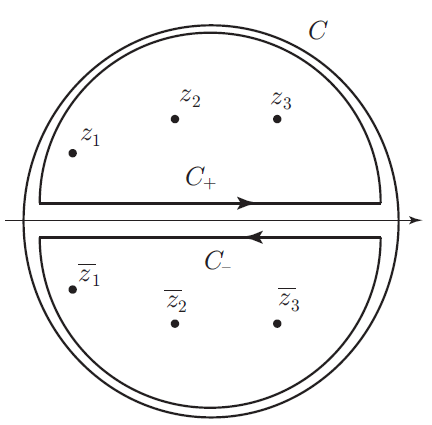
\includegraphics[width=0.6\linewidth]{fig/7.2.png}
	\caption{ $H$上CFT中$n$点函数的Ward恒等式。}
\end{figure}

无穷小共形变换由能动张量 $T_{\mu\nu} $生成。那么,变换不改变边界这一条件,就等价于能量和动量不流经边界。这条件用 $x,y$ 坐标写是 $T_{x y}=0$ ,用复坐标写是
\begin{equation}
	T_{x y}=\frac{1}{4 i}\left(T_{z z}-T_{\bar{z} \bar{z}}\right)=0 
\end{equation}
也就是说,在实轴上有
\begin{equation}
	T(z)=\bar{T}(\bar{z}), \quad z \in \mathbb{R}
\end{equation}
对实轴上取实值的全纯函数 $f(z)$ ,有
\begin{equation}
	f(\bar{z})=\overline{f(z)}
\end{equation} 
这是所谓\textbf{镜像原理}。因为$ \epsilon(z),T(z)$ 在实轴上取实值,它们可根据镜像原理延拓到下半复平面:
\begin{equation}
T(z)=\bar{T}(\bar{z}), \quad \epsilon(z)=\bar{\epsilon}(\bar{z}), \quad \operatorname{Im} z<0
\end{equation} 
因此, (7.22) 左边第二项线积分可改写到下半复平面$ H^{\prime}=\{z \in \mathbb{C}; \operatorname{Im} z<0\} $上:
$$
-\int_{C_{+}} d \bar{z} \frac{1}{2 \pi i} \bar{\epsilon}(\bar{z})\left\langle\bar{T}(\bar{z}) \phi_{1} \cdots \phi_{n}\right\rangle=\int_{C_{-}} d z \frac{1}{2 \pi i}\left\langle T(z) \phi_{1} \cdots \phi_{n}\right\rangle
$$
初级场在$ H'$ 上的位置,是点 $z_i $的复共轭点 $\bar{z}_{i} $,它们关于实轴镜像对称。闭合曲线 $C_- $是 $C_+ $的镜像。在Ward恒等式 (7.22) 中,实轴上的积分相互抵消了,只剩下围绕 $z_{1}, \bar{z}_{1}, \cdots, z_{n}, \bar{z}_{n} $的路径 $C$ 上的积分:
\begin{equation}
	\begin{aligned} & \int_{C} d z \frac{1}{2 \pi i} \epsilon(z)\left\langle T(z) \phi_{1} \cdots \phi_{n}\right\rangle \\ =&\sum_{i=1}^{n}\left(h_{i} \partial_{i} \epsilon\left(z_{i}\right)+\epsilon\left(z_{i}\right) \partial_{i}+h_{i} \partial_{i} \epsilon\left(\bar{z}_{i}\right)+\epsilon\left(\bar{z}_{i}\right) \partial_{i}\right)\left\langle\phi_{1} \cdots \phi_{n}\right\rangle \end{aligned}
\end{equation} 
这给出
\begin{equation}
	\begin{aligned} \left\langle T(z) \phi_{1} \cdots \phi_{n}\right\rangle=& \sum_{i=1}^{n}\left\{\frac{h_{i}}{\left(z-z_{i}\right)^{2}}+\frac{1}{z-z_{i}} \frac{\partial}{\partial z_{i}}+\frac{h_{i}}{\left(z-\bar{z}_{i}\right)^{2}}+\frac{1}{z-\bar{z}_{i}} \frac{\partial}{\partial \bar{z}_{i}}\right\} \\ & \times\left\langle\phi_{1} \cdots \phi_{n}\right\rangle \end{aligned}
\end{equation} 
这说明,上半复平面上 $n$ 点函数的共形Ward恒等式,等价于整个复平面上$ 2n$ 点函数的共形Ward恒等式。这种利用复共轭延拓到下半复平面,在整个复平面上处理的技术称为\textbf{加倍技巧(doubling trick)}。

例如, $H $上的单点函数$ \langle\phi(z, \bar{z})\rangle $等价于复平面上的两点函数$ \langle\phi(z) \phi(\bar{z})\rangle$ :
\begin{equation}
	\langle\phi(z, \bar{z})\rangle=\langle\phi(z) \phi(\bar{z})\rangle=\frac{A}{(2 y)^{2 h}}
\end{equation} \quad \quad (7.29)
$A $是常数。复平面上的单点函数,由共形对称性为零,$ H$ 上的则可非零。类似地, $H$ 上的两点函数$ \left\langle\phi\left(z_{1}, \bar{z}_{1}\right) \phi\left(z_{2}, \bar{z}_{2}\right)\right\rangle $等价于复平面上的四点函数$ \left\langle\phi\left(z_{1}^{\prime}\right) \phi\left(z_{2}^{\prime}\right) \phi\left(z_{3}^{\prime}\right) \phi\left(z_{4}^{\prime}\right)\right\rangle$ ,其中 $z_{1}^{\prime}=z_{1}, z_{2}^{\prime}=z_{2}, z_{3}^{\prime}=\bar{z}_{1} , z_{4}^{\prime}=\bar{z}_{2}$ 。引入交比
\begin{equation}
	\xi=\frac{z_{12}^{\prime} z_{34}^{\prime}}{z_{13}^{\prime} z_{24}^{\prime}}=\frac{\left(z_{1}-z_{2}\right)\left(\bar{z}_{1}-\bar{z}_{2}\right)}{\left(z_{1}-\bar{z}_{1}\right)\left(z_{2}-\bar{z}_{2}\right)}
\end{equation} 
(4.64) 给出
\begin{equation}
	\left\langle\phi\left(z_{1}, \bar{z}_{1}\right) \phi\left(z_{2}, \bar{z}_{2}\right)\right\rangle=\left(\frac{-1}{\left(z_{1}-\bar{z}_{1}\right)^{2}\left(z_{2}-\bar{z}_{2}\right)^{2}}\right)^{h} G_{43}^{21}(\xi)
\end{equation}
其中
\begin{equation}
	G_{43}^{21}(\xi)=\langle\phi(\infty) \phi(1) \phi(\xi) \phi(0)\rangle
\end{equation} 
注意,这里的交比 $\xi $和 (7.18) 定义的交比$ \eta$ 间的关系是
\begin{equation}
	\xi=\frac{\left(x_{1}-x_{2}\right)^{2}+\left(y_{1}-y_{2}\right)^{2}}{-4 y_{1} y_{2}}=\frac{\eta-1}{\eta} 
\end{equation}
此外,如果Virasoro代数有退化表示,可借助零模场得到关于$ G_{43}^{21}(\xi)$ 的解有固定奇点的微分方程,并由此得到关联函数。

例如,我们来计算Ising模型中自旋算符 $\sigma(z, \bar{z}) $的两点函数
$$
\left\langle\sigma\left(z_{1}, \bar{z}_{1}\right) \sigma\left(z_{2}, \bar{z}_{2}\right)\right\rangle
$$
它等价于复平面上的四点函数 (5.137) ,用这里的坐标写是
\begin{equation}
	\begin{aligned} &\left\langle\sigma\left(z_{1}\right) \sigma\left(z_{2}\right) \sigma\left(\bar{z}_{1}\right) \sigma\left(\bar{z}_{2}\right)\right\rangle \\ =&\left(\frac{\left(z_{1}-\bar{z}_{1}\right)\left(z_{2}-\bar{z}_{2}\right)}{\left(z_{1}-z_{2}\right)\left(\bar{z}_{1}-\bar{z}_{2}\right)\left(z_{1}-\bar{z}_{2}\right)\left(z_{2}-\bar{z}_{1}\right)}\right)^{\frac{1}{8}} F(\xi) \end{aligned} 
\end{equation}
共形块 $F(\xi)$ 是超几何微分方程 (5.138) 的解$ \sqrt{1 \pm \sqrt{1-\xi}}$ 的线性组合。于是
\begin{equation}
	\begin{aligned} \left\langle\sigma\left(z_{1}, \bar{z}_{1}\right) \sigma\left(z_{2}, \bar{z}_{2}\right)\right\rangle=&\left(\frac{1}{4 y_{1} y_{2}}\right)^{\frac{1}{8}} \xi^{-\frac{1}{8}}(1-\xi)^{-\frac{1}{8}} \\ & \times\left(a_{+} \sqrt{1+\sqrt{1-\xi}}+a_{-} \sqrt{1-\sqrt{1-\xi}}\right) \end{aligned}
\end{equation} 
$a_\pm $是常数。作为边界条件,我们要求实轴上$ \langle\sigma\rangle=0$ 。固定$ y_1,y_2$ , $\left|x_{1}-x_{2}\right| \rightarrow \infty $时两点函数趋于$ \langle\sigma\rangle\langle\sigma\rangle$ ,从而趋于零。这意味着,右边在 $\xi \rightarrow \infty $时趋于零,由此得到常数应当满足$ a_{+}-ia_{-} =0 $\footnote{J. L. Cardy, Nucl. Phys. B 240 (1984) 514.}。

\section{边界算符}
考虑借助加倍技巧延拓到整个复平面的能动张量 $T(z)$ 。它的模式展开系数定义为\textbf{边界Virasoro算符}
\begin{equation}
	L_{n}=\frac{1}{2 \pi i} \int_{C} d z z^{n+1} T(z) 
\end{equation}
$C $是围绕原点的闭合曲线。不像复平面上的CFT,边界Virasoro算符只有全纯部分。考虑边界Virasoro代数的Hilbert空间。

真空态 $|0\rangle$ 满足
\begin{equation}
	L_{n}|0\rangle=0, \quad(n \geq-1)
\end{equation} 
边界Virasoro算符最高权表示中的最高权态$ |h\rangle $满足
\begin{equation}
	L_{0}|h\rangle=h|h\rangle, \quad L_{n}|h\rangle=0, \quad(n \geq 1)
\end{equation} 
最高权态 $|h\rangle $对应初级场 $\psi(0) $,可由它作用在真空上得到:
\begin{equation}
	|h\rangle=\psi(0)|0\rangle 
\end{equation}
这里的初级场 $\psi(x)$ 是定义在边界(实轴)上的共形场, $x $是实数。定义在边界上的算符称为边界算符。通常定义在上半复平面上的算符$ \phi(z, \bar{z})$ 称为体算符。最高权态 $|h\rangle=\phi(0)|0\rangle $对应的$ L_0$ 的本征值称为边界共形维数。

由全局 $S L(2, \mathbb{R}) $共形对称性,可以确定边界共形维数为 $h_i$ 的边界初级场的关联函数:
\begin{align} &\left\langle\psi_{i}(x) \psi_{j}(y)\right\rangle=\frac{\delta_{i j} A_{i}}{|x-y|^{2 h_{i}}}\\ &\left\langle\psi_{i}\left(x_{1}\right) \psi_{j}\left(x_{2}\right) \psi_{k}\left(x_{3}\right)\right\rangle=\frac{C_{i j k}}{\left|x_{12}\right|^{h_{1}+h_{2}-h_{3}}\left|x_{23}\right|^{h_{2}+h_{3}-h_{1}}\left|x_{31}\right|^{h_{1}+h_{3}-h_{2}}} \end{align}
其中$ x_{i j}=x_{i}-x_{j}$ 。
\begin{figure}[h]
	\centering
	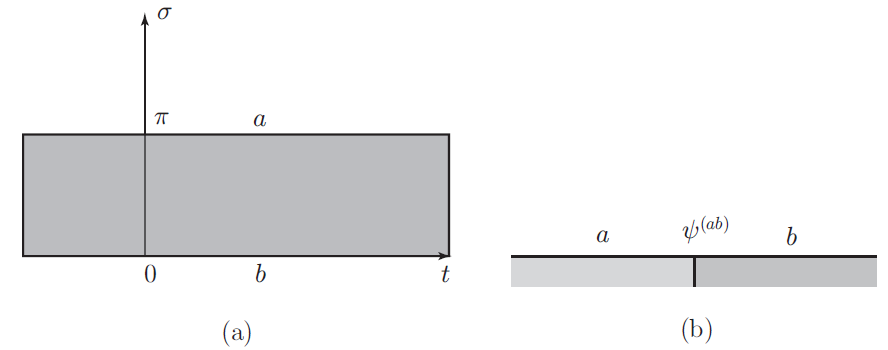
\includegraphics[width=0.6\linewidth]{fig/7.3.png}
	\caption{(a)带和边界条件。(b)连接边界条件$a$和$b$的边界算符$\psi^{(ab)}$。}
\end{figure}

在实轴上插入边界初级场会发生什么?我们用共形变换
\begin{equation}
	w=\log z=t+i \sigma
\end{equation} 
将上半复平面映成宽 $\pi $的无穷长带,如图7.3(a)。Hamiltonian是时间$ t $方向上的演化算符
\begin{equation}
	H=\int_{0}^{\pi} T_{t t} d \sigma-\frac{c}{24}
\end{equation}
6.1节讨论过,常数项来自Schwarz导数。借助加倍技巧,Hamiltonian可用边界Virasoro算符写成
\begin{equation}
	H=L_{0}-\frac{c}{24}
\end{equation} 
变换不改变边界这一条件,等价于 $T(z)=\bar{T}(\bar{z})$ ( $z\in\mathbb{R}$ ),用$ t,\sigma $坐标写是 $T_{t \sigma}=0$ ( $\sigma=0,\pi$ )。

边界条件有很多种。上下两边界上可以施加不同条件,确保仍然满足变换不改变边界这一条件即可。带上端(对应负半实轴)的边界条件记作$ a$ ,下端(对应正实半轴)的则记作 $b$ ,整个边界条件记作$ (ab)$ 。边界条件不同,意味着原点处不连续。在BCFT中,边界条件的变化可通过在$ z=0 $( $t=-\infty $)处插入边界初级场实现。对应边界条件$ (ab)$ 的边界初级场记作$ \psi^{(a b)}(x)$ ,如图7.3(b)。这种造成插入点左右边界条件不同的算符,有时称为边界改变算符。注意,恒等算符 $\boldsymbol{I}(x) $不会改变边界条件。\footnote{边界条件不同,也就破坏了原点处的平移对称性,这在径向量子化中意味着 $z=0 $处的“真空态”不再被$ L_{-1}$ 湮灭。根据态-算符对应,自然就相当于在 $z=0 $处插入算符。}

带边界条件 $(ab) $的系统的Hamiltonian记作 $H_{a b} $。$ H_{ab} $的本征空间可分解成边界Virasoro代数的不可约表示之和。最高权表示$ [h]$ 在分解中出现的次数记作 $n_{a b}^{h}$ 。满足$ n_{a b}^{h} \neq 0 $的最小的$ h $记作 $h_{ab}$ 。相应的边界初级场 $\psi^{(a b)}(x) $是基本的边界改变算符,$ h_{ab}$ 是它的边界共形维数。边界共形维数更高的场,可通过令其它算符作用在这个态上得到。特别地,在两侧边界条件相同的情形( a=b ),这个态是真空态 $|0\rangle$ ,对应恒等算符 $\boldsymbol{I}(x) $。 $h_{ab}=0$ , $[h_{ab}] $在分解中出现$ n_{a a}^{0}=1$ 次。\footnote{原书接下来的一句论证,我(\href{https://www.zhihu.com/people/wo-bei-56}{@笠道梓})不认同,发现文献中也有争议,因此按个人更认同的观点进行了改写。}

插入多个场时,我们只考虑最左侧和最右侧边界条件相同的情形,这相当于不在 $x=\pm \infty $处插入场,关联函数中就要出现额外的Kronecker delta符号。边界共形维数为 $h_i $的边界改变初级场 $\psi_{i}^{(a b)}(x)$ 的两点和三点函数是
\begin{align} &\left\langle\psi_{i}^{(a b)}(x) \psi_{j}^{(b c)}(y)\right\rangle=\frac{\delta_{i j} \delta_{a c} A_{i}^{a b}}{|x-y|^{2 h_{i}}}\\ &\left\langle\psi_{i}^{(a b)}\left(x_{1}\right) \psi_{j}^{(b c)}\left(x_{2}\right) \psi_{k}^{(c d)}\left(x_{3}\right)\right\rangle=\frac{\delta_{a d} C_{i j k}^{a b c}}{\left|x_{12}\right|^{h_{1}+h_{2}-h_{3}}\left|x_{23}\right|^{h_{2}+h_{3}-h_{1}}\left|x_{31}\right|^{h_{1}+h_{3}-h_{2}}} \end{align}

为确定这些三点函数中的系数,我们必须知道初级场OPE的结构。BCFT中的初级场包括体初级场$ \phi_{i}(z, \bar{z}) $和边界初级$场 \psi_{i}^{(a b)}(x)$ ,它们间的OPE都要纳入考虑。体初级场自身间的OPE和复平面上的形式相同,边界初级场自身间的OPE与上述两点和三点函数的结构一致。此外,体初级场靠近实轴时,同它的镜像生成了新的OPE。在BCFT中, $\phi_{i}(z, \bar{z})$ 的体共形权为 $\left(h_{i}, h_{i}\right)$ 时,OPE是(考虑自旋为零的场)\footnote{J. L. Cardy and D. C. Lewellen, Phys. Lett. B 259 (1991) 274.}\footnote{R. E. Behrend, P. A. Pearce, V. B. Petkova and J. B. Zuber, Nucl. Phys. B 570 (2000) 525 [arXiv:hep-th/9908036].}\footnote{I. Runkel, Nucl. Phys. B 549 (1999) 563 [arXiv:hep-th/9811178].}
\begin{align} &\phi_{i}(z, \bar{z}) \phi_{j}(w, \bar{w})=\sum_{k}|z-w|^{2\left(h_{k}-h_{i}-h_{j}\right)} C_{i j}^{k} \phi_{k}(w, \bar{w})\\ &\phi_{i}(z, \bar{z})=\sum_{k}{ }^{(a)} B_{i}^{k} \psi_{k}^{(a a)}(x)(2 y)^{h_{k}-2 h_{i}} \\ &\psi_{i}^{(a b)}(x) \psi_{j}^{(b c)}(y)=\sum_{k}(x-y)^{h_{k}-h_{i}-h_{j}} C_{i j}^{(a b c) k} \psi_{k}^{(a c)}(y) \end{align}
系数$ C_{i j}^{k}, {}^{(a)} B_{i}^{k}, C_{i j}^{(a b c) k}$ 表征着BCFT中的OPE。

\section{边界态}
在无穷长带的时间 $t $方向加上周期性:
$$
t \equiv t+2 \pi \delta
$$
就得到圆环,如图7.4。
\begin{figure}[h]
	\centering
	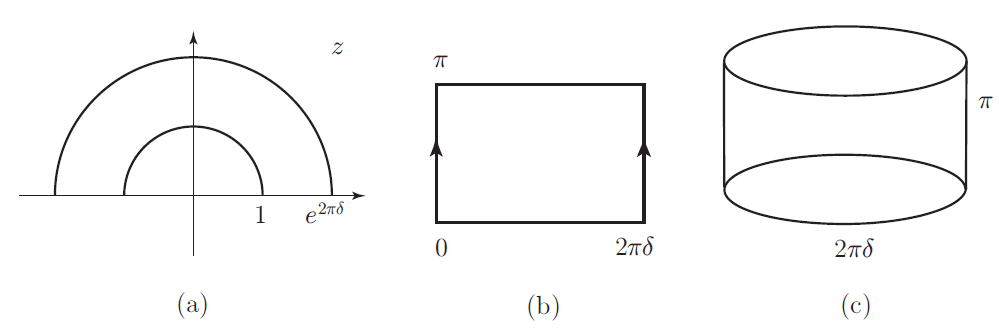
\includegraphics[width=0.6\linewidth]{fig/7.4.png}
	\caption{(a)$z$平面上的圆环,(b)长$2\pi \delta$,宽$\pi$的矩形,左右两边粘起来就得到圆环,(c)圆环。}
\end{figure}

这是一个带两条边界的曲面,如果再将这两条边界粘起来,就得到环面。

各边界条件记作$ a,b $,相应的Hamiltonian记作 $H_{ab} $,圆环上的配分函数是
\begin{equation}
	Z_{a b}(\delta)=\operatorname{Tr} e^{-2 \pi \delta H_{a b}} 
\end{equation}
因为Hamiltonian可用边界Virasoro算符写成 $H_{a b}=L_{0}-\frac{c}{24} $,它的本征空间可分解成边界Virasoro代数的最高权表示之和,我们有
\begin{equation}
	Z_{a b}(\delta)=\operatorname{Tr} q^{L_{0}-\frac{c}{24}}=\sum_{i} n_{a b}^{i} \chi_{h_{i}}(q)
\end{equation} 
这里$ q=e^{-2 \pi \delta} $。这对应将环面的模参数取成纯虚数 $\tau=i \delta $。$ \chi_{h_{i}}(q)=q^{-\frac{c}{24}} \operatorname{Tr}_{\left[h_{i}\right]} q^{L_{0}} $是边界Virasoro代数最高权表示$ [h_i]$ 的特征标, $n_{a b}^{i} $是$ [h_i] $在分解中出现的次数。

在环面的情形,配分函数模不变。特别地,将 $\tau $映成$ -1/\tau $的 $S $变换,交换了环面的时间和空间方向。在圆环的情形,模不变性对配分函数施加了什么限制呢?在 $S $变换下,
$$
q=e^{2 \pi i \tau} \rightarrow \tilde{q}=e^{-\frac{2 \pi i}{\tau}}=e^{-\frac{2 \pi}{\delta}}
$$
特征标的变换行为给出
\begin{equation}
	\chi_{h_{i}}(q)=\sum_{j} S_{i}^{j} \chi_{h_{j}}(\tilde{q})
\end{equation} 
于是配分函数是
\begin{equation}
	Z_{ab}=\sum_{i, j} n_{a b}^{i} S_{i}^{j} \chi_{h_{j}}(\tilde{q})
\end{equation} \quad \quad (7.53)
\begin{figure}[h]
	\centering
	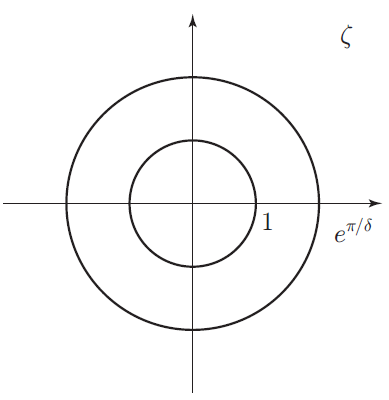
\includegraphics[width=0.6\linewidth]{fig/7.5.png}
	\caption{$\zeta$平面上的圆环。}
\end{figure}

另一方面,在圆环的情形,时间坐标 $t $和空间坐标 $\sigma $交换,周向成了空间方向,柱向则成了时间方向。变换后的Hamiltonian $H^{P} $是柱向的演化算符,我们用它来重写配分函数。共形变换
\begin{equation}
	\zeta=e^{-\frac{i}{\delta} w}=e^{-\frac{i}{\delta}(t+i \sigma)} 
\end{equation}\quad \quad (7.54)
下,图7.4(b)中的矩形映成图7.5中$ \zeta $平面上的圆环。为同之前的边界Virasoro算符区分,我们将$ \zeta$ 平面上的体Virasoro算符记作 $\hat{L}_{n}, \bar{\hat{L}}_{n}$ 。$ H^P $可用它们写成
\begin{equation}
	H^{P}=\hat{L}_{0}+\bar{\hat{L}}_{0}-\frac{c}{12}
\end{equation}
$\zeta$ 平面上的配分函数是从$ |\zeta|=1 $时的态$|a\rangle $到 $|\zeta|=e^{\frac{\pi}{\delta}} $时的态 $|b\rangle $的跃迁矩阵元
\begin{equation}
	Z_{ab}= \langle b |e^{-\frac{\pi}{\delta} H^{P}} | a \rangle= \langle b |\tilde{q}^{\frac{1}{2}\left(\hat{L}_{0}+\bar{\hat{L}}_{0}-\frac{c}{12}\right)} | a \rangle
\end{equation}
态 $|a\rangle,|b\rangle$ 称为\textbf{边界态},它们是Virasoro算符 $\hat{L}_{n}$, $\bar{\hat{L}}_{n}$ 作用的空间中的元素。

我们来进一步考察边界态的性质。能动张量可模式展开成
\begin{align} &\hat{T}(\zeta)=\sum_{n=-\infty}^{\infty} \hat{L}_{n} \zeta^{-n-2}\\ &\bar{\hat{T}}(\bar{\zeta})=\sum_{n=-\infty}^{\infty} \bar{\hat{L}}_{n} \bar{\zeta}^{-n-2} \end{align}
边界上\footnote{ z 平面上变换不改变边界的条件 (7.24) ,结合能动张量的变换行为 (3.52) 得到}$ \zeta^2\hat{T}(\zeta)-\bar{\zeta}^2\bar{\hat{T}}(\bar{\zeta})=0$ ,在边界 $|\zeta|=1 $上用相应的边界态 $|B\rangle $写是
\begin{equation}
	\left.(\zeta^2\hat{T}(\zeta)-\bar{\zeta}^2\bar{\hat{T}}(\bar{\zeta}))\right|_{|\zeta|=1}|B\rangle=0 
\end{equation}
用Virasoro算符写是
\begin{equation}
	\left(\hat{L}_{n}-\bar{\hat{L}}_{-n}\right)|B\rangle=0
\end{equation}

我们来在张量积空间 $[h] \otimes[\bar{h}]$ 中构造满足 (7.59) 的边界态 $|B\rangle $, $[h] $是$ \hat{L}_{n} $的最高权表示, $[\bar{h}] $是 $\bar{\hat{L}}_{n} $的最高权表示。注意,$ n=0$ 时,这个条件是
$$
\hat{L}_{0}|B\rangle=\bar{\hat{L}}_{0}|B\rangle
$$
这给出 $h=\bar{h}$ 。考虑$ [h]$ 级为 $N$ 的子空间,它的维数记作$d_{h}(N) $,标准正交基记作
$$
|h, N ; j\rangle, \quad j=1, \cdots, d_{h}(N)
$$
类似地,考虑 $[\bar{h}] $级为 $N $的子空间,标准正交基记作 $\overline{|h, N ; j\rangle} $。张量积空间的基从而是 $|h, N ; j\rangle\otimes\overline{|h, N ; j\rangle} $。引入满足
\begin{align} &U \overline{|h, 0\rangle}=\overline{|h, 0\rangle}^{*} \\ &U \bar{\hat{L}}_{n}=\bar{\hat{L}}_{n} U \end{align}
的反酉算符 $U $\footnote{反酉给出 $\langle Ux|Uy\rangle=\langle y|x\rangle$ },定义态
\begin{equation}
	|h\rangle\rangle=\sum_{N=0}^{\infty} \sum_{j=1}^{d_{h}(N)}|h, N ; j\rangle \otimes U \overline{|h, N ; j\rangle}
\end{equation}
这称为\textbf{Ishibashi态}\footnote{N. Ishibashi, Mod. Phys. Lett. A 4 (1989) 251.}。Ishibashi态是 $[h] \otimes[\bar{h}] $中 (7.59) 的唯一解。取 $\left(\hat{L}_{n}-\bar{\hat{L}}_{-n}\right)|h\rangle \rangle$ 和一般态 $\left\langle h, N_{1} ; k\right| \otimes U \overline{\left\langle h, N_{2} ; l\right|} $的内积,由基的标准正交性和算符的反酉性得到\footnote{由于$ h=\bar{h}$ ,相应表示中的矩阵元可以互相代换,我们有 $\langle x|A|y\rangle=\langle \bar{x}|\bar{A}|\bar{y}\rangle $。}
\begin{equation}
	\begin{aligned} & \left(\left\langle h, N_{1} ; k\right| \otimes U \overline{\left\langle h, N_{2} ; l\right|}\right)\left(\hat{L}_{n}-\bar{\hat{L}}_{-n}\right)|h\rangle \rangle \\ =& \sum_{N} \sum_{j}\left( \langle h, N_{1} ; k |\hat{L}_{n} | h, N ; j \rangle U \overline{\left\langle h, N_{2} ; l\right|} U \overline{|h, N ; j\rangle}\right.\\&\left.-\left\langle h, N_{1} ; k | h, N ; j\right\rangle U \overline{\left\langle h, N_{2} ; l\right|} \bar{\hat{L}}_{-n} U \overline{|h, N ; j\rangle}\right) \\ =& \langle h, N_{1} ; k |\hat{L}_{n} | h, N_{2} ; l \rangle- \langle h, N_{1} ;k |\hat{L}_{-n}^\dagger | h, N_{2} ; l \rangle \\ =& 0 \end{aligned}
\end{equation}
最后一个等号用了Hermite性$ \hat{L}_{-n}^{\dagger}=\hat{L}_{n}$ 。

Ishibashi态间的矩阵元可以算出是
\begin{equation}
	\begin{aligned} \langle \langle h^{\prime} |\tilde{q}^{\frac{1}{2}\left(\hat{L}_{0}+\bar{\hat{L}}_{0}-\frac{c}{12}\right)} | h \rangle \rangle=& \sum_{N^{\prime}=0}^{\infty} \sum_{j^{\prime}=1}^{d_{h^{\prime}}\left(N^{\prime}\right)} \sum_{N=0}^{\infty} \sum_{j=1}^{d_{h}(N)}\left\langle h^{\prime}, N^{\prime} ; j^{\prime}\right| \otimes U \bar{\left\langle h^{\prime}, N^{\prime} ; j^{\prime}\right|} \\ & \times \tilde{q}^{\frac{1}{2}\left(\hat{L}_{0}+\bar{\hat{L}}_{0}-\frac{c}{12}\right)}|h, N ; j\rangle \otimes U \overline{|h, N ; j\rangle} \\ =& \delta_{h^{\prime}, h} \sum_{N=0}^{\infty} \sum_{j=1}^{d_{h}(N)} \tilde{q}^{h+N-\frac{c}{24}} \\ =& \delta_{h^{\prime}, h} \sum_{N=0}^{\infty} d_{h}(N) \tilde{q}^{h+N-\frac{c}{24}} \\ =& \delta_{h, h^{\prime}} \chi_{h}(\tilde{q}) \end{aligned}
\end{equation} 
$\chi_{h}(\tilde{q}) $是Virasoro代数的特征标。

边界态 $|a\rangle $可用Ishibashi态展开成
\begin{equation}
	|a\rangle=\sum_{h}|h\rangle \rangle\langle\langle h |a\rangle
\end{equation}
代入配分函数 (7.56) 得到
\begin{equation}
	Z_{ab}=\sum_{h}\langle b | h\rangle \rangle \langle\langle h |a\rangle \chi_{h}(\tilde{q})
\end{equation} 
与 (7.53) 比对,我们得到矩阵元$ \langle\langle h |a\rangle $要满足
\begin{equation}
	\sum_{i} n_{b a}^{i} S_{i}^{j}=\left\langle b | h_{j} \rangle\right\rangle\left\langle\left\langle h_{j} |a\right\rangle\right.
\end{equation}
这称为\textbf{Cardy条件},满足这条件的边界态 $|a\rangle$ 称为\textbf{Cardy态}。

Virasoro代数最高权表示$ [h_j] $对应的边界条件记作 $\tilde{j}$ ,我们来构造边界态$ |\tilde{j}\rangle$ 。首先,恒等表示(记作$ j=0$ )对应的边界态记作 $|\tilde{0}\rangle$ 。这对应边界条件 $(\tilde{0}\tilde{0})$ ,Hamiltonian$ H_{\tilde{0} \tilde{0}}$ 的本征空间分解中只有恒等表示, $n_{\tilde{0} \tilde{0}}^{i}=\delta_{0}^{i} $,代入Cardy条件得到
\begin{equation}
	S_{0}^{j}= | \langle\tilde{0} |h_{j} \rangle \rangle |^{2}
\end{equation} 
这可写成
\begin{equation}
	|\tilde{0}\rangle=\sum_{j}\left(S_{0}^{j}\right)^{\frac{1}{2}} |h_{j} \rangle \rangle
\end{equation}
类似地,边界条件 $(\tilde{0}\tilde{l})$ ,对应Hamiltonian $H_{\tilde{0} \tilde{l}}$ 的本征空间分解中只有表示 $[h_l] $,对应边界态 $|\tilde{l}\rangle$ 。这时 $n_{\tilde{0} \tilde{l}}^{i}=\delta_{l}^{i}$ ,Cardy条件是
\begin{equation}
	S_l^j=\langle \tilde{0}|h_j\rangle\rangle\langle\langle h_j|l\rangle
\end{equation}
即
\begin{equation}
	\langle \langle h_{j} | \tilde{l} \rangle=\frac{S_{l}^{j}}{\left(S_{0}^{j}\right)^{1 / 2}} 
\end{equation}
于是
\begin{equation}
	|\tilde{l}\rangle=\sum_{j} \frac{S_{l}^{j}}{\left(S_{0}^{j}\right)^{1 / 2}}\left|h_{j}\right\rangle \rangle
\end{equation}
此外,取 $n_{\tilde{l} \tilde{0}}^{i}=\delta_{l}^{i}$ 给出左矢
\begin{equation}
	\langle\tilde{l}|=\sum_{j} \frac{\left(S_{l}^{j}\right)^{*}}{\left(S_{0}^{j}\right)^{1 / 2}}\left\langle\left\langle h_{j}\right|\right. 
\end{equation}
为方便,再定义
\begin{equation}
	\langle\tilde{l}^{\vee} |=\sum_{j} \frac{S_{l}^{j}}{\left(S_{0}^{j}\right)^{1 / 2}} \langle\left\langle h_{j}\right| 
\end{equation}
在极小模型的情形,模$ S $矩阵实对称,不必区分它们。

以Ising模型为例。由模 $S$ 矩阵 (6.139) , $h=0,1/2,1/16$ 初级态对应的Ishibashi态记作 $|0\rangle\rangle,|\epsilon\rangle\rangle,|\sigma\rangle\rangle$ ,那么Cardy态是
\begin{equation}
	\begin{aligned} & |\tilde{0}\rangle=\frac{1}{\sqrt{2}}|0\rangle \rangle+\frac{1}{\sqrt{2}}|\epsilon\rangle \rangle+\frac{1}{2^{\frac{1}{4}}}|\sigma\rangle \rangle \\ & \left|\frac{\tilde{1}}{2}\right\rangle=\frac{1}{\sqrt{2}}|0\rangle \rangle+\frac{1}{\sqrt{2}}|\epsilon\rangle \rangle-\frac{1}{2^{\frac{1}{4}}}|\sigma\rangle \rangle \\ & \left|\frac{\tilde{1}}{16}\right\rangle=|0\rangle \rangle-|\epsilon\rangle \rangle \end{aligned}
\end{equation}
用Ising模型的语言来说, $|\tilde{0}\rangle $是自旋向上的边界态, $\left|\frac{\tilde{1}}{2}\right\rangle$ 是自旋向下的边界态, $\left|\frac{\tilde{1}}{16}\right\rangle $是自由边界条件,由此我们记
\begin{equation}
	\begin{aligned} &|+\rangle=|\tilde{0}\rangle \\ &|-\rangle=\left|\frac{\tilde{1}}{2}\right\rangle \\ &|f\rangle=\left|\frac{\tilde{1}}{16}\right\rangle \end{aligned} 
\end{equation}
各边界条件下的配分函数是
\begin{align} &Z_{++}=Z_{--}=\frac{1}{2} \chi_{0}+\frac{1}{2} \chi_{\frac{1}{2}}+\frac{1}{\sqrt{2}} \chi_{\frac{1}{16}} \\ &Z_{f f}=\chi_{0}+\chi_{\frac{1}{2}}\\ &Z_{+-}=\frac{1}{2} \chi_{0}+\frac{1}{2} \chi_{\frac{1}{2}}-\frac{1}{\sqrt{2}} \chi_{\frac{1}{16}}\\ &Z_{+f}=Z_{-f}=\frac{1}{\sqrt{2}} \chi_{0}-\frac{1}{\sqrt{2}} \chi_{\frac{1}{2}} \end{align}

\subsection{BCFT和Verlinde公式}
Cardy态的表达式代入Cardy条件得到
\begin{equation}
	\sum_{i} S_{i}^{j} n_{\tilde{k}^{\vee} \tilde{l}}^{i}=\frac{S_{k}^{j} S_{l}^{j}}{S_{0}^{j}}
\end{equation} 
如果这里的 $n_{\tilde{k}^{\vee} \tilde{l}}^{i} $等于融合系数 $N_{k l}^{i}$ ,那么这个式子就是Verlinde公式 (6.167) 。
\begin{figure}[h]
	\centering
	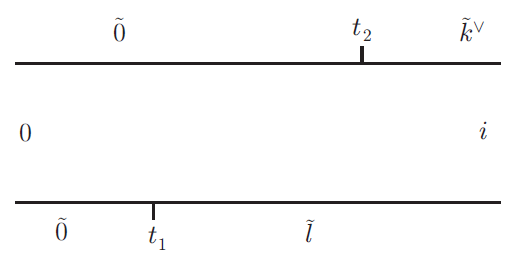
\includegraphics[width=0.6\linewidth]{fig/7.6.png}
	\caption{带上的BCFT和Verlinde公式。}
\end{figure}

Cardy从BCFT的角度给出了Verlinde公式的解释\footnote{J. L. Cardy, Nucl. Phys. B 324 (1989) 581.}。考虑带上的BCFT,假定某些时刻边界条件发生了改变,如图7.6。 $t<t_1 $时边界条件是 $(\tilde{0}\tilde{0})$ 。 $t=t_1$ 时下端的边界条件从 $\tilde{0}$ 变为 $\tilde{l}$ ,这相当于插入边界算符 $\psi_{\tilde{l} \tilde{0}} $。那么Hamiltonian从 $H_{\tilde{0} \tilde{0}} $变为$ H_{\tilde{l} \tilde{0}} $,$ n_{b a}^{i}$ 从 $n_{\tilde{0} \tilde{0}}^{i}=\delta_{0}^{i}$ 变为 $n_{\tilde{0} \tilde{l}}^{i}=\delta_{l}^{i} $,这相当于融合系数从 $N_{00}^{i}=\delta_{0}^{i} $变为 $N_{l 0}^{i}=\delta_{l}^{i}$ 。 $t=t_2>t_1$ 时上端的边界条件从 $\tilde{0} $变为 $\tilde{k}^{\vee} $,这相当于插入边界算符 $\psi_{\tilde{k} ^\vee \tilde{0}}$ ,那么 $n_{b a}^{i}$ 从 $n_{\tilde{l}\tilde{0}}^{i} $变为$ n_{\tilde{k}^{\vee} \tilde{l}}^{i} $。这个数等于表示 $k^{\vee} $对应的场和表示$ l$ 对应的场组合起来再分解时,表示$ i $对应的场出现的次数,就是融合系数 $N_{k l}^{i}$ 。




